\documentclass[12pt, a4paper]{article}

\usepackage[czech]{babel}
%\usepackage[IL2]{fontenc}
\usepackage[utf8]{inputenc}
\usepackage{enumitem}
\usepackage{parskip}
\usepackage{tocloft}
\usepackage{multicol}
\usepackage[hidelinks]{hyperref}
\usepackage{graphicx}
\usepackage{float}
\usepackage{listings}
\usepackage{xcolor}

% Define code style for C
\lstset{
    language=C,
    basicstyle=\ttfamily,
    keywordstyle=\color{blue},
    stringstyle=\color{red},
    commentstyle=\color{green},
    breaklines=true
    frame=shadowbox,
    numbers=left,
    numberstyle=\small,
    stepnumber=1,
    numbersep=5pt,
    showstringspaces=false,
    tabsize=4,
    captionpos=b,
}


\begin{document}

%Uvodni strana
\begin{titlepage}
    
\includegraphics[width=0.75\textwidth]{img/fav.png}
    \begin{center}
        
        
        \vspace{2cm}
        
        \Huge
        Semestrální práce KIV/ZOS
        
        \vspace{1cm}
        
        \LARGE
        Základy operačních systémů
        
        \vfill
        
        \vspace{0.5cm}
        
        \normalsize
        \raggedright
        Student:        Adam Míka \\
        Osobní číslo:   A22B0319P \\
        Email:          mikaa@students.zcu.cz \\
        Datum:          20. září 2024
        \vspace{0.2cm}
        
    \end{center}
\end{titlepage}

%tečky v obsahu
\renewcommand{\cftsecleader}{\cftdotfill{\cftdotsep}}
\renewcommand{\cftsubsecleader}{\cftdotfill{\cftdotsep}}
\renewcommand{\cftsubsubsecleader}{\cftdotfill{\cftdotsep}}

%obsah
\setcounter{page}{2}
\tableofcontents
\listoffigures
\lstlistoflistings
\begin{thebibliography}{99}
    \bibitem{image1ref} Zdroj Obrázku 1: \url{https://philipstel.wordpress.com/2010/08/04/dictionary-based-algorithm-lempel-ziv-welch/}
  \end{thebibliography}
\pagebreak


\section{Zadání}
\large
\textbf{Hlavní cíle:}
\normalsize
Zbytek zadání zde: \href{https://portal.zcu.cz/CoursewarePortlets2/DownloadDokumentu?id=238432}{\textcolor[RGB]{20,20,200}{\underline{\textit{PDF}}}}


\section{Analýza úlohy}

Úkolem této práce je navrhnout a implementovat komunikační protokol pro hru „Rock-Paper-Scissors“ (kámen, nůžky, papír) v rámci předmětu KIV/UPS. Hra je koncipována pro více hráčů, konkrétně pro dva účastníky, kteří spolu soutěží v sérii 10 kol. Každé kolo probíhá tak, že oba hráči nezávisle na sobě zvolí jednu z možností (kámen, nůžky, nebo papír) a poté tuto volbu odešlou serveru. Server následně zpracuje přijaté tahy, vyhodnotí výsledek daného kola, určí vítěze, aktualizuje skóre obou hráčů a případně ukončí hru po odehrání všech kol.

\subsection{Popis protokolu}

Komunikační protokol zahrnuje různé typy zpráv, které slouží pro přenos informací mezi klientem a serverem. Každý typ zprávy má specifickou strukturu a účel. Níže jsou popsány jednotlivé typy zpráv použité v protokolu:

\begin{itemize}
    \item \textbf{PlayMessage}: Tato zpráva je odesílána klientem, když hráč zvolí svůj tah (kámen, nůžky, nebo papír). Obsahuje identifikátor hry, identifikátor hráče a zvolenou akci.
    \item \textbf{ValidMoveMessage}: Server touto zprávou potvrzuje, že přijal platný tah od daného hráče.
    \item \textbf{ResultMessage}: Tato zpráva je odesílána serverem, aby informovala o výsledku daného kola. Zahrnuje informace o tahu obou hráčů a výsledku (výhra, prohra, remíza).
    \item \textbf{RoundEndMessage}: Server touto zprávou oznamuje ukončení aktuálního kola a poskytuje aktuální skóre obou hráčů.
    \item \textbf{GameEndMessage}: Tato zpráva informuje o ukončení hry a oznamuje celkového vítěze nebo důvod předčasného ukončení hry (např. dosažení maximálního počtu kol).
    \item \textbf{ExitMessage}: Zpráva slouží k indikaci odpojení hráče nebo ukončení hry ze strany klienta či serveru.
\end{itemize}

Každá zpráva obsahuje hlavičku, která je tvořena následujícími položkami:
\begin{itemize}
    \item \textbf{magic}: Konstantní řetězec „KIVRPS“, který slouží k identifikaci protokolu.
    \item \textbf{command}: Typ příkazu, který specifikuje, o jaký druh zprávy se jedná (např. „play“, „result“).
    \item \textbf{totalLength}: Celková délka zprávy.
\end{itemize}

\subsection{Diagram protokolu}

Na obrázku \ref{fig:protocol} je znázorněn diagram komunikačního protokolu, který zobrazuje strukturu zpráv a vztahy mezi nimi. Tento diagram slouží jako vizuální reprezentace, která usnadňuje pochopení způsobu výměny informací mezi klientem a serverem.

\begin{figure}[H]
    \centering
    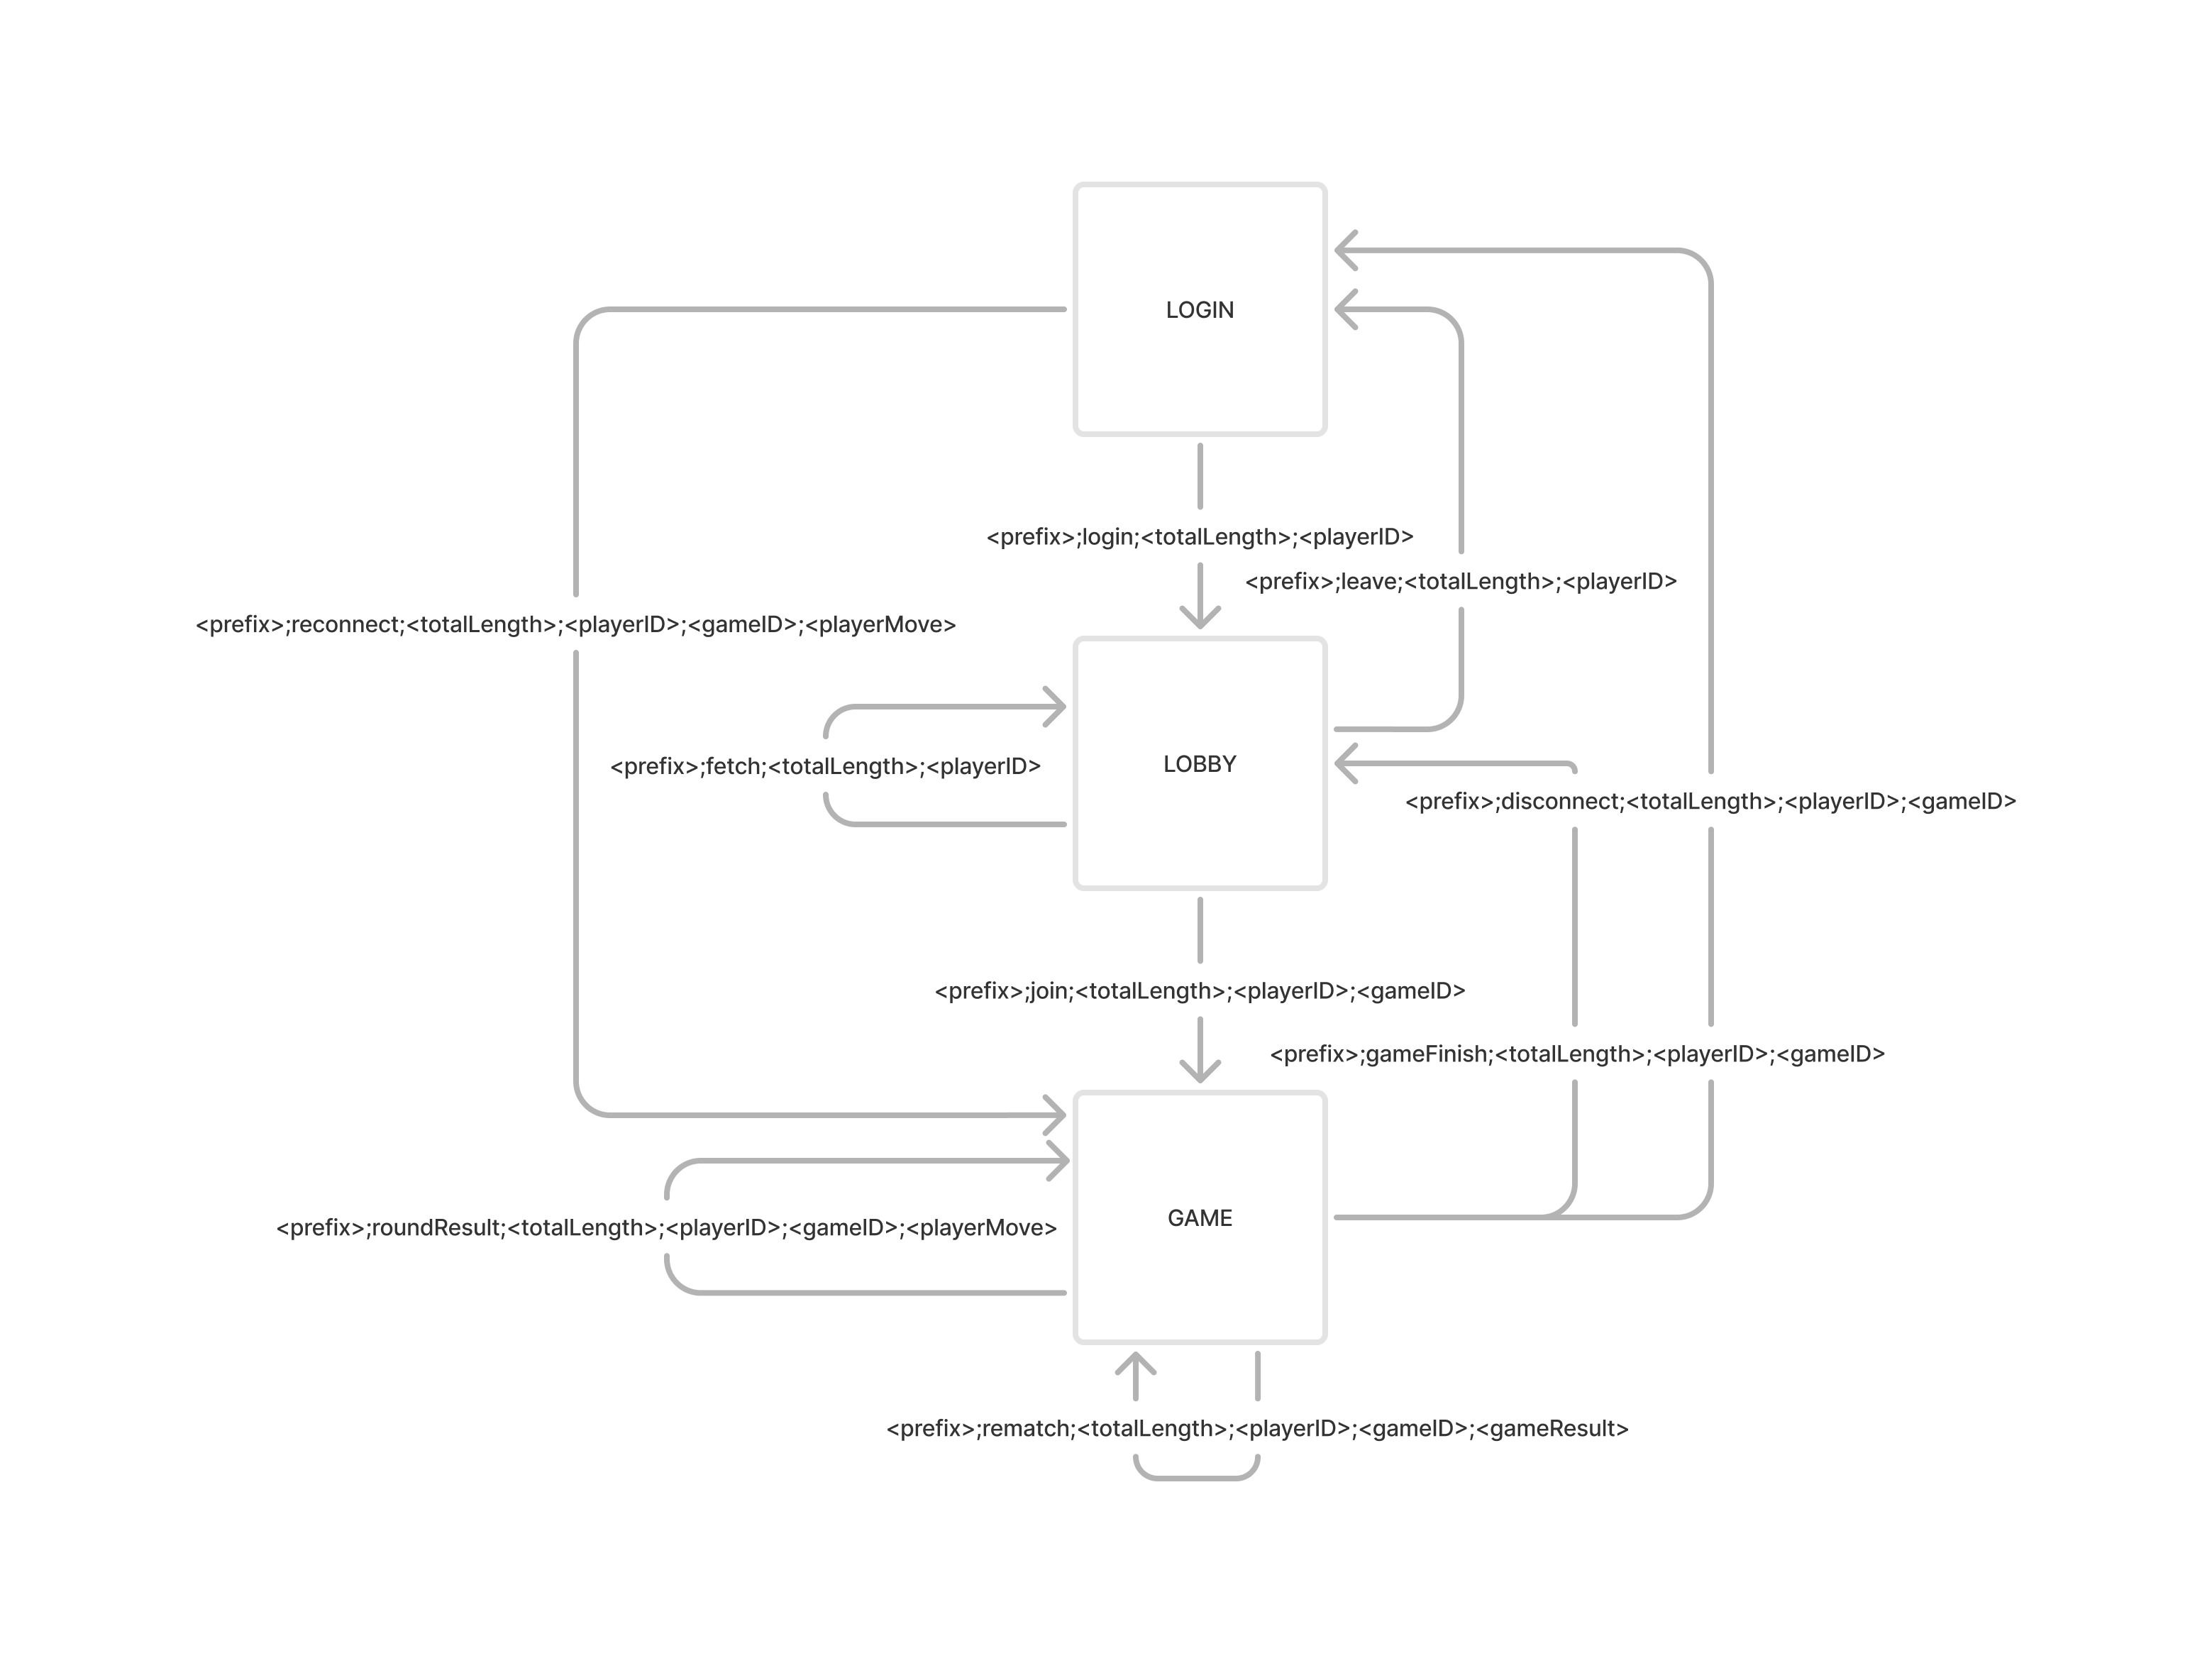
\includegraphics[width=0.7\textwidth]{img/protocol.png}
    \caption{Diagram komunikačního protokolu pro hru Rock-Paper-Scissors}
    \label{fig:protocol}
\end{figure}

Navržený protokol zajišťuje efektivní přenos informací a synchronizaci průběhu hry. Díky použití standardu ASN.1 lze protokol snadno rozšířit a přizpůsobit pro případné další požadavky na funkcionalitu systému.


\section{Ipmlementace}

\begin{lstlisting}
// hello.c
#include <stdio.h>

int main() {
    printf("Hello, World!\n");
    return 0;
}
\end{lstlisting}


\section{Uživatelská příručka}


\section{Závěr}

\end{document}
